\subsection{System Model}\label{sec:application:lte_video:system_model}
In this section, we present modeling assumptions used in the remainder of this section.
Then, we propose a system model for both video transmission mechanisms and the considered \gls{LTE} network.
Finally, we introduce performance metrics for each of the considered stakeholders.

\subsubsection*{Model Assumptions}\label{sec:application:lte_video:system_model:model_assumptions}
Maintaining a high \gls{QoE} for their viewers is an important goal for operators of video platforms.
The authors of~\cite{Hossfeld2012a} find that the \gls{QoE} is mainly influenced by the number of stalling events and the stalling event duration.
As shown in \reffig{fig:application:lte_video:system_model:stalling2qoe}, the \gls{QoE} model, where 5 is the highest possible \gls{MOS} and 1 the lowest, rapidly decreases if the number or duration of stalling events increases.
The provided \gls{QoE} model between stalling and \gls{QoE} shows that stalling significantly worsens \gls{QoE}.
Thus, an operator has to avoid stalling at any cost.
As a consequence, we only consider scenarios where no stalling occur, i.e. the delivery bandwidth is larger than the minimum video bitrate to ensure a smooth video playout.
Furthermore, in \refsec{sec:application:qoe_user_behaviour} we will study the impact of available network load and user preference on \gls{QoE}.

\begin{figure}
  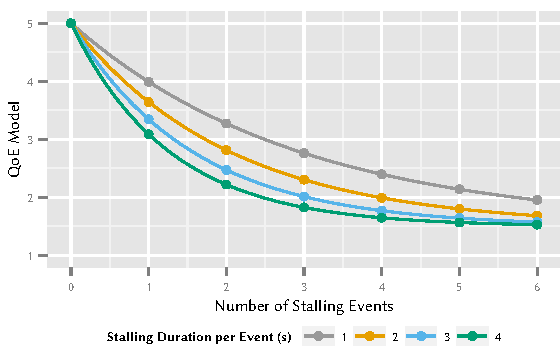
\includegraphics{application/lte_video/system_model/figures/stalling2qoe}
  \caption{Influence of number of stalling events and stalling length on \headershortacr{QoE}~\cite{Hossfeld2012a}.}
  \label{fig:application:lte_video:system_model:stalling2qoe}
\end{figure}

Furthermore, we assume that all videos are played back with a constant bitrate \(\bitrate\).
Thus, each second of the video, independently of its content, requires the same number of bits.

We consider video transmission between a server and a user equipped with an \gls{LTE} enabled smartphone.
The available bandwidth of a \gls{UE} depends on many factors, e.g. location, number of users in the cell, activity of other users, and line of sight.
To simplify the evaluation scenarios we assume that a constant maximum bandwidth \(\bandwidth\) is provided to the user.
We assume that the bottleneck of the connection is the air interface, thus the full available bandwidth \(\bandwidth\)  is used for the video download, which prevents stalling.

Although the assumptions of constant bitrate and bandwidth do not hold in a real environment, the purpose of considering such assumptions is twofold.
First, they are useful in order to analyse the performance of the discussed mechanisms in optimal conditions without any other effects that could disturb the results and, second, they can serve as a baseline for comparison with fitted random variables for both bandwidth and bitrate.

\subsubsection*{Video Traffic Model}\label{sec:application:lte_video:system_model:video_traffic}

In our study we focus on four transmission mechanisms which are currently in use.
\reffig{fig:application:lte_video:system_model:video_model:playback} shows the consumed bandwidth \(\bandwidthdown(t)\) and the available seconds of video for playback \(\timeunwatched(t)\) for a video for all considered transmission mechanisms at all points of time \(t\).
Furthermore, for the remainder of this chapter, we refer to the amount of video in seconds already played back at a point in time \(t\) as \(\timeplayedback(t)\).

\begin{figure}
	\begin{subfigure}[b]{\textwidth}
	\centering
	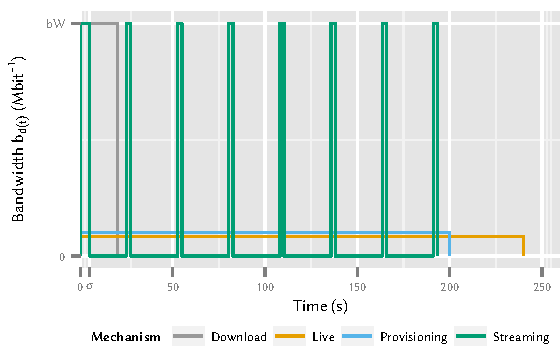
\includegraphics{application/lte_video/system_model/figures/video_model_bandwidth}
	\caption{Bandwidth consumption \(\bandwidth\)}\label{fig:application:lte_video:system_model:video_model:bandwidth}
	\end{subfigure} 
	\begin{subfigure}[b]{\textwidth}
	\centering
	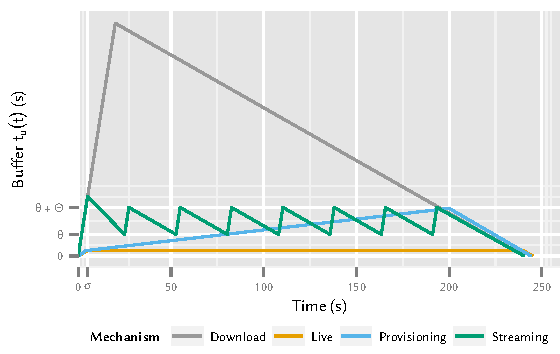
\includegraphics{application/lte_video/system_model/figures/video_model_playback}
	\caption{Remaining playback buffer \(\timeunwatched(t)\)}\label{fig:application:lte_video:system_model:video_model:playback}
	\end{subfigure}

	\caption{Behaviour of transmission mechanisms. Different playback end times occur due to different playback starts.}\label{fig:application:lte_video:system_model:video_model}
\end{figure}

\begin{enumerate}
\item \textbf{\download} The \emph{\download} mechanism can be used if a user wants to watch a pre-encoded video.
Thus, the complete video is ready to be transmitted as soon as the user starts the transmission.
The required time of the download is only bounded by the bandwidth available in the network.

\item \textbf{\live} Video watched during \emph{\live} transmissions is encoded as it is recorded.
Thus, the bandwidth used to transmit the video is always limited to the video bitrate \bitrate.

\item \textbf{\serviceprovisioning} In~\cite{Hossfeld2011a} the authors show the influence of the video demand, i.e. the ratio of available bandwidth and required video bandwidth, on the stalling frequency.
In order to reduce stalling, the bandwidth used to download the video should be provisioned so that the available bandwidth exceeds the video bandwidth by a high enough factor.
In the \emph{\serviceprovisioning} mechanism, the download bandwidth is chosen so no stalling occurs.
In order to reduce stalling and improve the \gls{QoE} of a video, the available bandwidth should be at least \SI{120}{\percent} of the video bitrate \bitrate~\cite{Hossfeld13a}.

\item \textbf{\streaming} For the \emph{\streaming} mechanism the complete video is encoded in advance, allowing for the full bandwidth of the \gls{UE} being used for download.
The video is downloaded with full bandwidth for a \emph{prebuffering time} \streamingstart in order to guarantee a stalling-free start of the playback.
After \(\streamingstart\) \si{\second} the download stops and the playback begins.
The download is only resumed if the available seconds of video for playback are below a \emph{stop threshold} \bufferlower.
The download continues until the buffer contains a \emph{threshold size} \buffersize, resulting in a total buffer length of \(\bufferlower + \buffersize\) \si{\second}.
This is repeated until the download is completed.
\end{enumerate}

A video provider will also consider its bandwidth to be a resource to be conserved.
However, when comparing the bandwidth available in \gls{LTE} with that of a wired network, we can assume the air interface to be the bottleneck.
Furthermore, not considering bandwidth as an optimisation target of the video provider simplifies the study as it removes one additional metric.

\subsubsection*{\headershortacr{LTE} Network Model}\label{sec:application:lte_video:system_model:lte_network_model}
In order to quantify the energy consumption during wireless transmission, we model the \gls{LTE} \gls{RRC} behaviour defined in~\cite{3GPP_RRC_Spec}.
To reduce the energy consumption, the concept of \gls{DRX} has been introduced in~\cite{3GPP_MAC}.
The authors of~\cite{Huang2012} provide measurements of important \gls{RRC} and \gls{DRX} parameters which are used in the following model and are reproduced in \reftab{tab:application:lte_video:system_model:lte_network_model:rrc_drx_parameters}.

\begin{table}
  \begin{center}
    \begin{tabular}{lcc}
    \toprule
    Full Name & Symbol & Measured Value\\
    \midrule
    \rrcconnected \emph{On} duration timer & \ton & \SI{1}{\milli\second}\\
    \gls{DRX} inactivity timer & \tdrxinactivity & \SI{100}{\milli\second}\\
    \shortdrx duration timer & \tshortdrx & \SI{20}{\milli\second}\\
    \longdrx duration timer & \tlongdrx & \SI{40}{\milli\second}\\
    \rrcconnected timeout & \tidle & \SI{11.576}{\second} \\
    \rrcidle \emph{On} duration timer & \tonidle & \SI{43}{\milli\second}\\
    \rrcidle \gls{DRX} duration timer & \tdrxidle & \SI{1.28}{\second}\\
    Promotion Delay & \promotiondelay & \SI{260}{\milli\second}\\
	\bottomrule
    \end{tabular}
  \end{center}
  \caption{Considered \headershortacr{RRC} and \headershortacr{DRX} parameters~\cite{Huang2012}.}
  \label{tab:application:lte_video:system_model:lte_network_model:rrc_drx_parameters}
\end{table}

\begin{figure}
\begin{center}
  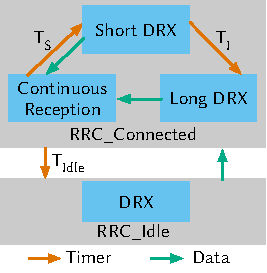
\includegraphics{application/lte_video/system_model/figures/model_lte}
  \caption{Considered \headershortacr{LTE} \headershortacr{RRC} model.}
  \label{fig:application:lte_video:system_model:lte_network_model:model_lte}
\end{center}
\end{figure}

The \gls{RRC} protocol for \gls{LTE} consists of two states, as shown in \reffig{fig:application:lte_video:system_model:lte_network_model:model_lte}.
In \rrcidle state, the \gls{UE} is in \gls{DRX} mode.
Here, the \gls{UE} monitors the \gls{PDCCH} for \tonidle in each \gls{DRX} interval of duration \tdrxidle.
The time of a promotion to the \rrcconnected state is given by the promotion delay \promotiondelay and occurs as soon as a packet is sent or received.
If a packet is sent or received while in \rrcconnected, including the initial packet which triggered the promotion to \rrcconnected, the timers \tdrxinactivity and \tidle are started.
Until the \tdrxinactivity timer expires, the \gls{UE} is in \gls{CRX} mode.
After the \tidle timer expires, the \gls{UE} demotes to \rrcidle.
Upon expiration of the \tdrxinactivity timer, the \gls{UE} enters \shortdrx.
Here, the \tshortdrx timer is started and the \gls{UE} monitors \gls{PDCCH} for \ton.
If a packet is sent or received while in \shortdrx, \gls{CRX} begins and the \tshortdrx timer is disabled.
Once the \tshortdrx timer expires, \longdrx is entered and \tlongdrx is started, again the \gls{UE} monitors \gls{PDCCH} for \ton.
This is repeated until a packet is sent or received and the \gls{CRX} state is entered or until the \tidle timer expires and \rrcidle is entered.

We give the download bandwidth at any time \(t\) as \(\bandwidthdown(t)\), as shown in \reffig{fig:application:lte_video:system_model:video_model:bandwidth}.
Furthermore, we denote the length of the video already downloaded at any time \(t\) as 
\begin{equation}
\timedownloaded(t) = \frac{1}{\bitrate} \int_{\tau=0}^t \bandwidthdown(\tau) d\mathrm{\tau}.
\end{equation}

\subsubsection*{Evaluation Metrics for Smartphone Energy Consumption, Wasted Traffic, and Connection Count}\label{sec:application:lte_video:system_model:model_assumptions:metrics}
Each of the stakeholders is interested in different \glspl{KPI}, from which we derive a set of metrics considered during the performance evaluation of the network and video playback model.

\paragraph*{Energy Consumption}
We calculate the power drain of the \gls{UE} due to wireless transmission at any given moment using the \gls{UE}'s current state and the bandwidth in use and aggregate it to the \gls{UE}'s energy consumption during the duration of the video playback.
We only consider the energy consumption due to wireless transmission, as it is an offset to the energy consumption caused by the playback of the video.
The video playback itself is unaffected by the choice of transmission mechanism.
Thus, the selected transmission mechanism only influences the energy consumption of the wireless transmission.
In~\cite{Huang2012}, the authors provided measurements for the energy consumption of each state, reproduced in \reftab{tab:application:lte_video:system_model:model_assumptions:metrics:power_parameters}, if the \gls{UE} is receiving no data.
Furthermore, an approximation of the power drain at time \(t\) if a download occurs is given as 
\[\power(t) =\factordown \cdot \bandwidthdown(t) + \powerbaseline.\]
In order to compute the overall energy consumption \(\energyconsumption\) during the transmission and playback of the video, we aggregate the power consumed in each state in which the \gls{UE} is not receiving and the power consumed during receiving while considering the used bandwidth at each moment.

\begin{table}
  \begin{center}
    \begin{tabular}{lc}
    \toprule
    Description & Power drain\\
    \midrule
    \rrcidle (base) & \SI{11.4}{\milli\watt}\\
    \gls{DRX} during \rrcidle & \SI{594.3}{\milli\watt}\\
    Promotion & \SI{1210.7}{\milli\watt}\\
    \rrcconnected (base) & \SI{1060.0}{\milli\watt}\\
    \gls{DRX} during \shortdrx & \SI{1680.2}{\milli\watt}\\
    \gls{DRX} during \longdrx & \SI{1680.1}{\milli\watt}\\
    \factordown & \SI{51.97}{\milli\watt\per\mega\bit}\\
    \powerbaseline & \SI{1288.04}{\milli\watt}\\
    \bottomrule
    \end{tabular}
  \end{center}
  \caption{Power consumption per system state~\cite{Huang2012}.}
  \label{tab:application:lte_video:system_model:model_assumptions:metrics:power_parameters}
\end{table}

\paragraph*{Wasted Traffic}
If a user stops watching a video currently being downloaded before its end, this leads to \emph{wasted traffic} as the data has been already prebuffered at the \gls{UE}.
This metric impacts the video provider, but is influenced by the user aborting the video.
This decision can not be influenced by the video provider, thus a user model has to be assumed by the video provider in order to provide a performance analysis of the different video delivery mechanisms.

Considering that transmitting data to a smartphone costs both money and traffic, a transmission mechanism should attempt to reduce the amount of video which has been transmitted but is not yet watched at any time \(t\) as 
\[\timeunwatched(t) = \timedownloaded(t) - \timeplayedback(t)\]
If the user stops the playback according to a random variable \userabortrv with \gls{PDF} \(\userabortpdf\), we can give the wasted traffic \meanwastedtraffic as the expected value of $\timeunwatched$ under $\userabortrv$.
\begin{equation}
\meanwastedtraffic = E\left[\timeunwatched\right] = \int_{t=0}^{\infty} \userabortpdf(t) \timeunwatched(t) d\mathrm{t}.
\end{equation}
High values of \meanwastedtraffic indicate that server and network resources are used for traffic which is not watched by the user.

\begin{figure}
\begin{center}
  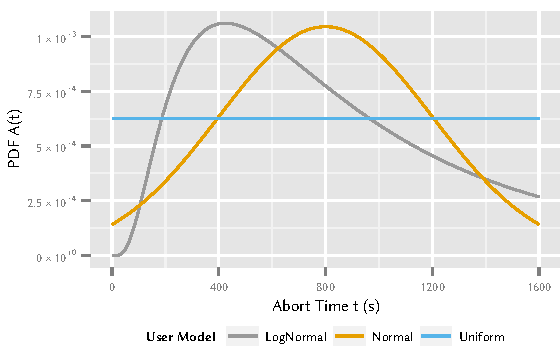
\includegraphics{application/lte_video/system_model/figures/abort_distributions}
  \caption{Considered user model abort distributions.}
  \label{fig:application:lte_video:system_model:model_assumptions:metrics:abort_distributions}
\end{center}
\end{figure}

We consider three types of user behaviour, shown in \reffig{fig:application:lte_video:system_model:model_assumptions:metrics:abort_distributions}, each modeled by a random variable describing the abort time, i.e. the time when the user stops watching a video.
First we consider a \emph{uniform} distributed user abort model, where the user can abort the video at any time.
Due to the uniform distribution of the abort time and the length of the video, i.e. \SI{1600}{\second}, the mean time of stop occurs at \SI{800}{\second}.

Second, we consider a type of user that watches a part of the video before deciding if the video is stopped. 
After the main part of the video has been watched, the user is again more likely to abort.
To model this kind of behaviour we use a \emph{truncated normal distribution} over the playtime of the video, assuming a symmetry of the abort density at the half-way point of the video.
We use the same mean and specify a standard deviation of \SI{400}{\second}.

Finally, we assume that the user is more likely to abort the video at the beginning.
We model this user behaviour using a \emph{truncated log-normal distribution} with the same mean and a standard deviation of \SI{0.8}{\second} for the normal distribution at the basis of the log-normal distribution.

Note that the wasted traffic \meanwastedtraffic is influenced by the user abort model, due to the fact that wasted traffic only occurs if a user aborts a video.
Even though this may only affect a subset of all watched videos, it still consumes unnecessary resources and should be considered by the video provider.
However, the download of videos always consumes energy and the largest amount of energy is consumed if the user does not abort the video.
Thus, we optimise for the worst case energy consumption.
Any other optimisation target would offer incentives to users to abort watching the video early, resulting in additional wasted traffic for the provider.

\paragraph*{Connection Count}
A large portion of signalling messages caused by data transmission are generated if the \gls{UE} switches between connected and disconnected state~\cite{3GPP_RRC_Spec}.
Thus, counting the number of connections \connectioncount triggered provides an easy way to quantify the generated signalling during the video transmission.
